% =====================================================================
%  Лекция 3. Описательная статистика. Статистики 1-го типа.
%  Дата: 2026-10-01
% =====================================================================
\section{Описательная статистика. Статистики 1-го типа}
\label{lec:03}

% Структура лекции: \subsection — тема, \subsubsection — её подтемы.
\subsection{Описательная статистика}
\label{lec03:descriptive}

\emph{Описательная статистика}~--- набор графиков и числовых характеристик
генеральной совокупности~$\xi$, найденных по имеющейся выборке $X_{[n]}$,
а также всевозможные функции от выборки, которые характеризуют случайную величину.

\subsubsection{Размах и эмпирические моменты}

\begin{example}
  \label{lec03:range}
  Разность между максимальным и минимальным значениями выборки
  \[
    R(X_{[n]}) = X_{\max} - X_{\min} = X_{(n)} - X_{(1)}
  \]
  называется \emph{размахом выборки}. Здесь $X_{(1)}$ и $X_{(n)}$~--- порядковые статистики.
\end{example}

\begin{example}
  \label{lec03:moments}
  Эмпирические моменты:
  \begin{align*}
    a_k^{*}   &= \frac{1}{n} \sum_{i=1}^n X_i^k
              && \text{начальный эмпирический момент порядка } k, \\
    a_1^{*}   &= \frac{1}{n} \sum_{i=1}^n X_i = \Xbar
              && \text{выборочное среднее}, \\
    a_k^{0*}  &= \frac{1}{n} \sum_{i=1}^n (X_i - \Xbar)^k
              && \text{центральный эмпирический момент порядка } k, \\
    a_2^{0*}  &= \frac{1}{n} \sum_{i=1}^n (X_i - \Xbar)^2 = s^2
              && \text{выборочная дисперсия}, \\
    \tilde{s}^2 &= \frac{n}{n-1}\, s^2
              && \text{исправленная дисперсия}.
  \end{align*}
\end{example}

\subsubsection{Квантили и медиана}

\begin{definition}
  \emph{Выборочным квантилем порядка} $p \in (0, 1)$ называется элемент
  вариационного ряда $X_{(1)} \le \ldots \le X_{(n)}$ с номером $[np] + 1$,
  где $[a]$~--- целая часть числа~$a$:
  \[
    x_p = X_{([np] + 1)}.
  \]
\end{definition}

Выборочный квантиль~--- эмпирический аналог квантиля распределения:
\emph{квантилем порядка}~$p$ случайной величины~$\xi$ называется число~$u_p$,
для которого $F_\xi(u_p) = p$ (см.~\cref{lec03:fig:quantile}).

\begin{figure}[h]
  \centering
  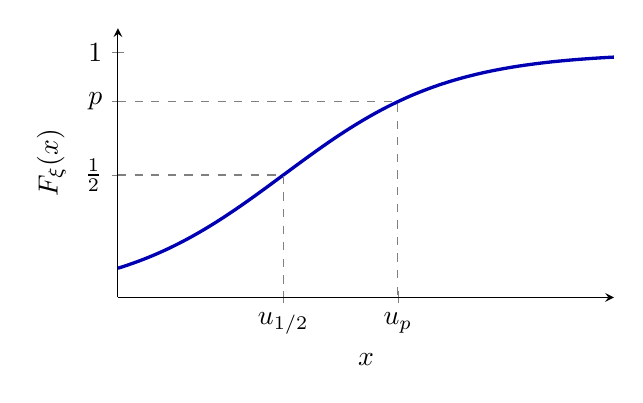
\begin{tikzpicture}
    \begin{axis}[
      width=0.65\textwidth, height=5cm,
      xmin=0, xmax=6, ymin=0, ymax=1.1,
      axis lines=left, xlabel={$x$}, ylabel={$F_\xi(x)$},
      xtick={2, 3.386}, xticklabels={$u_{1/2}$, $u_p$},
      ytick={0.5, 0.8, 1}, yticklabels={$\frac12$, $p$, $1$},
    ]
      \addplot[very thick, blue!70!black, domain=0:6, samples=100] {1/(1 + exp(-(x - 2)))};
      \addplot[dashed, gray] coordinates {(0, 0.5) (2, 0.5) (2, 0)};
      \addplot[dashed, gray] coordinates {(0, 0.8) (3.386, 0.8) (3.386, 0)};
    \end{axis}
  \end{tikzpicture}
  \caption{Квантили распределения: $F_\xi(u_p) = p$; $u_{1/2}$~--- медиана.}
  \label{lec03:fig:quantile}
\end{figure}

Частные случаи:
\begin{itemize}
  \item \emph{процентили}~--- $p = 0{,}01;\ 0{,}02;\ \ldots;\ 0{,}99$;
  \item \emph{децили}~--- $p = 0{,}1;\ 0{,}2;\ \ldots;\ 0{,}9$;
  \item \emph{квартили}~--- $p = 0{,}25;\ 0{,}5;\ 0{,}75$.
\end{itemize}

Квартили обозначают $Q_1$, $Q_2$, $Q_3$:
\begin{itemize}
  \item $Q_1 = x_{0{,}25}$~--- \emph{первый квартиль}: 25\,\% элементов
        выборки меньше него и 75\,\% больше;
  \item $Q_2 = x_{0{,}5}$~--- \emph{второй квартиль}, или \emph{выборочная медиана};
  \item $Q_3 = x_{0{,}75}$~--- \emph{третий квартиль}: 75\,\% элементов
        выборки меньше него и 25\,\% больше.
\end{itemize}

\begin{definition}
  \emph{Выборочной медианой} называется число, которое делит вариационный ряд
  на две части, содержащие равное количество элементов:
  \[
    \operatorname{med} X_{[n]} =
    \begin{dcases}
      X_{(k+1)},                  & \text{если } n = 2k + 1, \\
      \frac{X_{(k)} + X_{(k+1)}}{2}, & \text{если } n = 2k.
    \end{dcases}
  \]
\end{definition}

\begin{example}
  Пусть $n = 100$, $p = 0{,}5$. Выборочный квантиль имеет номер $[np] + 1 = 51$,
  то есть $x_{0{,}5} = X_{(51)}$, а выборочная медиана равна
  $\dfrac{X_{(50)} + X_{(51)}}{2}$.
\end{example}

\begin{remark}
  Для несимметричных данных (например, с длинным правым хвостом) выборочное
  среднее смещается в сторону хвоста, а медиана к нему устойчива. Поэтому для
  таких данных медиана лучше описывает <<центр>> выборки.
\end{remark}

\begin{definition}
  \emph{Межквартильным размахом} называется величина
  \[
    \mathrm{IQR} = Q_3 - Q_1.
  \]
\end{definition}

Между $Q_1$ и $Q_3$ лежит примерно половина элементов выборки.

\subsubsection{Мода и полигон частот}

\begin{definition}
  \emph{Выборочной модой} называется элемент выборки, который встречается
  чаще всего. Если таких элементов несколько, то мода не определена.
\end{definition}

\emph{Группированные данные.} Если вариационный ряд $X_{(1)} \le \ldots \le X_{(n)}$
разбит на интервалы длины~$l_i$ (как при построении гистограммы) и $\nu_i$~---
число элементов выборки в $i$-м интервале, то можно построить
\emph{полигон относительных частот}~--- ломаную с вершинами в точках
$\bigl(\tilde{x}_i,\ \nu_i / (n l_i)\bigr)$, где $\tilde{x}_i$~--- середина $i$-го интервала.
Вершины полигона~--- середины верхних сторон столбцов гистограммы относительных частот.

\subsubsection{Асимметрия и эксцесс}

\begin{definition}
  \emph{Коэффициентом асимметрии} называется величина
  \[
    A_s = \frac{a_3^{0*}}{s^3}
        = \frac{\frac{1}{n} \sum_{i=1}^n (X_i - \Xbar)^3}
               {\Bigl(\frac{1}{n} \sum_{i=1}^n (X_i - \Xbar)^2\Bigr)^{3/2}},
  \]
  то есть третий центральный эмпирический момент, делённый на куб
  среднеквадратического отклонения.
\end{definition}

Если $A_s > 0$, то распределение скошено вправо (длинный правый хвост),
если $A_s < 0$~--- влево. Для симметричного распределения теоретический
коэффициент асимметрии равен нулю.

\begin{definition}
  \emph{Коэффициентом эксцесса} называется величина
  \[
    E_k = \frac{a_4^{0*}}{s^4} - 3.
  \]
  Это эмпирический аналог теоретического коэффициента эксцесса
  \[
    \frac{\E (\xi - \E\xi)^4}{(\D\xi)^2} - 3.
  \]
\end{definition}

Для нормального распределения теоретические коэффициенты асимметрии
и эксцесса равны нулю.

\medskip

Все эти характеристики строят, чтобы примерно определить вид распределения
генеральной совокупности.

\subsection{Статистики первого типа}
\label{lec03:first-type}

Статистика~--- это любая борелевская функция на выборочном пространстве
(см.~лекцию~\ref{lec:01}). Нас будет интересовать более узкий класс~--- статистики первого типа.

Пусть задана случайная величина~$\xi$ и выборка $X_{[n]} = (X_1, \ldots, X_n)$
из генеральной совокупности~$\xi$. Пусть заданы борелевские функции
\[
  g \colon \R \to \R^m, \qquad h \colon \R^m \to \R^l,
\]
и существует \emph{конечный} интеграл
\[
  a \eqdef \int_{-\infty}^{+\infty} g(x)\, dF_\xi(x) = \E g(\xi)
  = \bigl(\E g_1(\xi), \ldots, \E g_m(\xi)\bigr) \in \R^m,
\]
причём $h$ непрерывна в точке~$a$.

На множестве функций распределения~$F$ определим функционал
\[
  G(F) = h\biggl(\int_{-\infty}^{+\infty} g(x)\, dF(x)\biggr).
\]
В частности, $G(F_\xi) = h(a)$.

\begin{definition}
  \emph{Статистикой первого типа} называется статистика
  \[
    S(X_{[n]}) = G(F_n^*),
  \]
  где $F_n^*$~--- эмпирическая функция распределения.
\end{definition}

То есть $S$~--- это функционал~$G$, вычисленный на эмпирическом распределении.
Распишем его:
\[
  S(X_{[n]})
  = h\biggl(\int_{-\infty}^{+\infty} g(x)\, dF_n^*(x)\biggr)
  = h\biggl(\frac{1}{n} \sum_{i=1}^{n} g(X_i)\biggr).
\]
Почему второе равенство: интеграл здесь~--- интеграл Лебега--Стилтьеса, а функция
$F_n^*(x) = \nu\bigl((-\infty, x]\bigr)/n$ кусочно-постоянна.
Она растёт только скачками в точках выборки, и в каждой точке $X_i$ скачок равен~$\frac1n$.
При интегрировании по такой функции значение $g$ в точке скачка умножается на величину
скачка, поэтому
\[
  \int_{-\infty}^{+\infty} g(x)\, dF_n^*(x) = \sum_{i=1}^{n} g(X_i) \cdot \frac{1}{n}.
\]

\begin{remark}
  Если среди $X_1, \ldots, X_n$ есть совпадающие значения, скачки не все одинаковые:
  в точке, где совпали $k$ элементов выборки, скачок равен $\frac{k}{n}$.
  Формула от этого не меняется~--- просто $g$ в этой точке входит в сумму $k$ раз.
\end{remark}

\begin{example}
  Пусть $h(t) = t$, $h \colon \R \to \R$, и $g(x) = x^k$. Тогда
  \[
    S(X_{[n]}) = \frac{1}{n} \sum_{i=1}^{n} X_i^k = a_k^*,
  \]
  то есть начальный эмпирический момент порядка~$k$ является статистикой первого типа.
  В частности, при $k = 1$ получаем $S(X_{[n]}) = \Xbar$.
\end{example}

Значит, любой начальный выборочный момент~--- статистика первого типа.
Центральные моменты $a_k^{0*}$ тоже: если раскрыть $(X_i - \Xbar)^k$ по биному,
$a_k^{0*}$ выразится многочленом от $a_1^*, \ldots, a_k^*$, и этот многочлен можно взять
в качестве~$h$, а $g(x) = (x, x^2, \ldots, x^k)$. Пример для $k = 2$ далее:

\begin{example}
  Пусть $\E\xi^2 < \infty$ и
  \[
    g(x) = (x, x^2), \quad g \colon \R \to \R^2, \qquad
    h(t) = t_2 - t_1^2, \quad h \colon \R^2 \to \R.
  \]
  Функция $h$~--- многочлен, поэтому она непрерывна всюду, в том числе в точке
  $a = (\E\xi, \E\xi^2)$. Тогда
  \[
    G(F_\xi) = h(a) = \E\xi^2 - (\E\xi)^2 = \D\xi,
  \]
  а соответствующая статистика первого типа~--- выборочная дисперсия:
  \[
    S(X_{[n]})
    = \frac{1}{n} \sum_{i=1}^{n} X_i^2 - \biggl(\frac{1}{n} \sum_{i=1}^{n} X_i\biggr)^{\!2}
    = a_2^* - (a_1^*)^2
    = \frac{1}{n} \sum_{i=1}^{n} (X_i - \Xbar)^2
    = s^2.
  \]
  Последнее равенство следует из того, что
  $\frac1n \sum_{i=1}^n (X_i - \Xbar)^2 = \frac1n \sum_{i=1}^n X_i^2 - 2\Xbar^2 + \Xbar^2$.
  Таким образом, $s^2$~--- эмпирический аналог дисперсии $\D\xi$.
\end{example}

\begin{theorem}
  \label{lec03:first-type-conv}
  Если $S(X_{[n]}) = G(F_n^*)$~--- статистика первого типа, то
  \[
    S(X_{[n]}) \toas h(a) = G(F_\xi) \quad \textup{при } n \to \infty,
  \]
  или, в другой записи,
  \[
    G(F_n^*) \toas G(F_\xi) \quad \textup{при } n \to \infty.
  \]
\end{theorem}

\begin{reminder}[УЗБЧ Колмогорова (теорема~\ref{lec02:slln})]
  Пусть $\xi_1, \xi_2, \ldots$~--- независимые одинаково распределённые случайные
  величины, $\E\abs{\xi_1} < \infty$. Тогда
  \[
    \frac{1}{n} \sum_{i=1}^{n} \xi_i \toas \E\xi_1 \quad \textup{при } n \to \infty.
  \]
\end{reminder}

\begin{proof}
  Напомним, что $S(X_{[n]}) = h\bigl(\frac{1}{n} \sum_{i=1}^{n} g(X_i)\bigr)$.
  Доказательство разбивается на два шага.

  \emph{Шаг 1: к $g(X_i)$ применим УЗБЧ.} Проверим условия для каждой компоненты
  $g_j(X_i)$, $j = 1, \ldots, m$:
  \begin{itemize}
    \item $g_j(X_i)$~--- случайная величина, так как $g$ борелевская;
    \item $g_j(X_1), g_j(X_2), \ldots$ независимы: борелевские функции от независимых
          случайных величин независимы;
    \item они одинаково распределены: все $X_i$ распределены как~$\xi$, значит,
          все $g_j(X_i)$ распределены как $g_j(\xi)$;
    \item $\E\abs{g_j(\xi)} < \infty$: это и есть условие конечности $a$ из определения.
  \end{itemize}
  Все условия УЗБЧ выполнены, поэтому для каждой компоненты
  $\frac{1}{n} \sum_{i=1}^{n} g_j(X_i) \toas \E g_j(\xi) = a_j$, то есть
  \[
    \frac{1}{n} \sum_{i=1}^{n} g(X_i) \toas a.
  \]
  Обозначим через $A$ событие, на котором эта сходимость выполняется; $\P(A) = 1$.

  \emph{Шаг 2: непрерывность $h$.} Зафиксируем $\omega \in A$. Тогда
  $\frac{1}{n} \sum_{i=1}^{n} g\bigl(X_i(\omega)\bigr)$~--- обычная числовая
  последовательность в $\R^m$, сходящаяся к~$a$. Функция $h$ непрерывна в точке~$a$,
  поэтому по определению непрерывности по Гейне
  $h\bigl(\frac{1}{n} \sum_{i=1}^{n} g(X_i(\omega))\bigr) \to h(a)$.
  Это верно для всех $\omega \in A$, а $\P(A) = 1$, следовательно,
  \[
    S(X_{[n]}) = h\biggl(\frac{1}{n} \sum_{i=1}^{n} g(X_i)\biggr) \toas h(a) = G(F_\xi). \qedhere
  \]
\end{proof}

\begin{remark}
  Непрерывность $h$ нужна только в точке~$a$: предел $\frac{1}{n} \sum_{i=1}^{n} g(X_i)$~---
  неслучайная точка~$a$, и значения $h$ вдали от неё на сходимость не влияют.
  Борелевость $h$ нужна для другого~--- чтобы $S(X_{[n]})$ была случайной величиной,
  то есть статистикой.
\end{remark}

\begin{example}
  Предположим, что
  \[
    g(x) = x^k, \quad g \colon \R \to \R, \qquad
    h(t) = t, \quad h \colon \R \to \R.
  \]
  Тогда $a_k^* = h(\frac{1}{n} \sum_{i=1}^{n} g(X_i)) \toas \E\xi^k = a_k$.
  То есть $k$-й эмперический момент сходится почти наверное к $k$-му теоретическому моменту.
\end{example}

Аналогичная сходимость выполняется и для центральных моментов, дисперсии, коэффициентов асимметрии и эксцесса.

\subsubsection{Двумерная выборка: ковариация и корреляция}

До сих пор выборка была последовательностью независимых случайных величин.
Теперь пусть это последовательность независимых случайных \emph{векторов}.
Для простоты возьмём двумерный случай: $\xi = (\xi_1, \xi_2)$~--- случайный вектор и
\[
  X_{[n]} =
  \begin{pmatrix}
    X_{11} & \ldots & X_{1n} \\
    X_{21} & \ldots & X_{2n}
  \end{pmatrix},
\]
где столбцы $(X_{1i}, X_{2i})$ независимы и распределены как~$\xi$.

\begin{reminder}
  \emph{Ковариация} и \emph{коэффициент корреляции} (Пирсона):
  \[
    \cov(\xi_1, \xi_2) = \E(\xi_1 - \E\xi_1)(\xi_2 - \E\xi_2) = \E\xi_1\xi_2 - \E\xi_1\,\E\xi_2,
    \qquad
    \rho(\xi_1, \xi_2) = \frac{\cov(\xi_1, \xi_2)}{\sqrt{\D\xi_1}\,\sqrt{\D\xi_2}}.
  \]
  Коэффициент корреляции показывает степень \emph{линейной} связи.
  Из независимости следует некоррелированность ($\rho = 0$), но не наоборот.
\end{reminder}

\begin{definition}
  Пусть $\Xbar_j = \frac1n \sum_{i=1}^n X_{ji}$ и
  $s_j = \sqrt{\frac1n \sum_{i=1}^n (X_{ji} - \Xbar_j)^2}$, $j = 1, 2$.
  \emph{Выборочной ковариацией} и \emph{выборочным коэффициентом корреляции} называются
  \[
    \widehat{\cov}(\xi_1, \xi_2) = \frac1n \sum_{i=1}^n (X_{1i} - \Xbar_1)(X_{2i} - \Xbar_2),
    \qquad
    \hat\rho(\xi_1, \xi_2) = \frac{\widehat{\cov}(\xi_1, \xi_2)}{s_1 s_2}.
  \]
\end{definition}

\begin{proposition}
  $\widehat{\cov}$ и $\hat\rho$~--- статистики первого типа.
\end{proposition}

\begin{proof}
  Раскрывая скобки, получаем
  \[
    \widehat{\cov}(\xi_1, \xi_2)
    = \frac1n \sum_{i=1}^n X_{1i} X_{2i}
      - \biggl(\frac1n \sum_{i=1}^n X_{1i}\biggr)\biggl(\frac1n \sum_{i=1}^n X_{2i}\biggr).
  \]
  Это $h\bigl(\frac1n \sum g(X_{1i}, X_{2i})\bigr)$ при
  $g(x, y) = (x,\, y,\, xy)$ и $h(t) = t_3 - t_1 t_2$.
  Для $\hat\rho$ берём $g(x, y) = (x,\, y,\, x^2,\, y^2,\, xy)$ и
  \[
    h(t) = \frac{t_5 - t_1 t_2}{\sqrt{(t_3 - t_1^2)(t_4 - t_2^2)}}.
  \]
  Обе $h$ непрерывны в точке~$a$ (для $\hat\rho$~--- при $\D\xi_1, \D\xi_2 > 0$,
  чтобы знаменатель в точке~$a$ не обращался в ноль).
\end{proof}

\begin{corollary}
  Если $\E\xi_1^2, \E\xi_2^2 < \infty$ и $\D\xi_1, \D\xi_2 > 0$, то при $n \to \infty$
  \[
    \widehat{\cov}(\xi_1, \xi_2) \toas \cov(\xi_1, \xi_2),
    \qquad
    \hat\rho(\xi_1, \xi_2) \toas \rho(\xi_1, \xi_2).
  \]
\end{corollary}